\chapter{Two-source Fourier Transform Spectroscopy}
\label{chap:refractive_index}

\section{Introduction}
\label{intro_ts}
In chapter \ref{chap:two_source}, the $0-\pi$ square-wave phase grating (SWPG) was introduced as a means of generating two intense duplicates of an input femtosecond mid-IR pulse.  An additional element of the SWPG is that it enables precise control over the relative phase between these two sources.  When used to generate high harmonics, this scheme enables the generation of two XUV sources whose relative phase is well controlled by the SWPG, and any small phase shift between the two harmonic beams is imprinted upon their interference pattern as a fringe shift in the far-field.  The idea is to now leverage this sensitivity to measure an induced phase shift between the two XUV sources.  In the experiment described in this chapter, the phase shift will be induced by introducing a thin condensed matter sample into only one of the two XUV sources.  Doing so enables us to extract both the real and imaginary part of the refractive index over a broad range of photon energies in the XUV.
\section{Complex refractive index}
The complex refractive index depends strongly on photon energy, and a cartoon of this is shown in figure \ref{fig:refractive_index_schematic}. We are interested in the refractive index in the XUV energy region, and in this region there are many resonances that correspond to transitions of core-level electrons to unoccupied states near the Fermi level (for the case of a condensed matter system)\cite{stohrNEXAFSSpectroscopy1992, attwoodSoftXraysExtreme2000}.  Complicated fine structure can emerge near these resonances that correspond to the local electronic and geometric environment\cite{stohrNEXAFSSpectroscopy1992, attwoodSoftXraysExtreme2000}.  Thus, the ability to measure both the real and imaginary parts of the complex refractive index can be important for many experiments using XUV light generated by HHG\cite{kaplanFemtosecondTrackingCarrier2018,  cirriAchievingSurfaceSensitivity2017}.

\begin{figure}
	\centering
	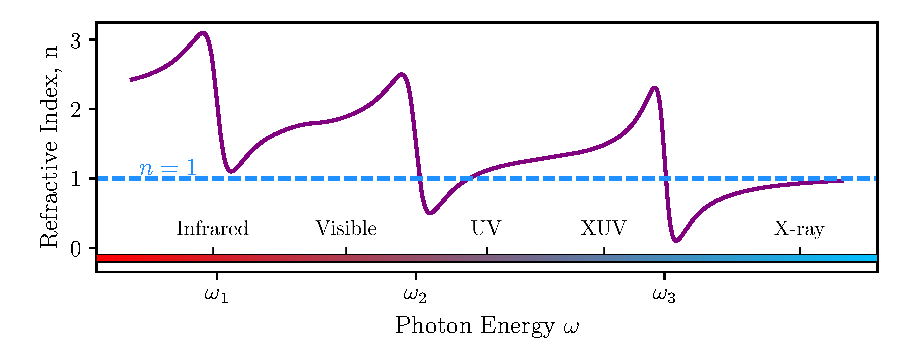
\includegraphics[width=1.0\textwidth]{figures/refractive_index/example_refractive_index.pdf}
	\caption[Schematic of real part of the refractive index from infrared to X-ray wavelengths]{Schematic of the real part of the refractive index versus photon energy. Example resonances are shown in the IR, the visible/UV, and in the XUV/soft x-ray regimes. In general, the refractive index approaches 1 at higher photon energies.}
	\label{fig:refractive_index_schematic}
\end{figure}

In general, the complex refractive index can be written as
\begin{equation}
\label{eqn:refractive_index}
	n(\omega)=1 - \bigg(\frac{n_a r_e \lambda^2}{2\pi}\bigg)\bigg[f_1(\omega) - i f_2(\omega)\bigg]
\end{equation}
where $f_1$ and $f_2$ are the atomic scattering factors, $n_a$ is the number density, $\omega$ ($\lambda$) is the photon energy (wavelength), and
\begin{equation}
\label{eqn:r_e}
	r_e = \frac{e^2}{4\pi\epsilon_0 mc^2}
\end{equation}
is the classical electron radius \cite{attwoodSoftXraysExtreme2000}. By introducing the parameters $\beta$ and $\delta$, such that
\begin{equation}
\label{eqn:delta_beta_def}
	\begin{aligned}
	\delta &= \frac{n_a r_e \lambda^2}{2\pi}f_1(\omega)\\
	\beta & = \frac{n_a r_e \lambda^2}{2\pi}f_2(\omega),
	\end{aligned}
\end{equation}
then the refractive index $n$ can be written as
\begin{equation}
\label{eqn:refractive_index_db}
	n(\omega)=1-\delta+i\beta.
\end{equation}
The values of both $\delta$ and $\beta$ have been tabulated for elements up to uranium in the range of 10 eV to 30 keV\cite{henkeLowenergyXrayInteraction1982}, and their values are generally smaller than unity when far from resonance.

Now that we've established the form of the refractive index, we will consider the case of propagation through a dispersive medium and its effect on amplitude and phase of a wave \cite{attwoodSoftXraysExtreme2000}. The idea is to consider a plane wave of the form
\begin{equation}
	\mathbf{E}(\mathbf{r},t)=\mathbf{E}_0e^{-i(\omega t - \mathbf{k}\cdot\mathbf{r})},
\end{equation}
and assume that the dispersion of the medium takes the form
\begin{equation}
	\frac{\omega}{k}=\frac{c}{1-\delta+i\beta}.
\end{equation}
With these relationships, one can write the field in the propagation direction defined by $\mathbf{k}\cdot\mathbf{r}=kr$ as
\begin{equation}
\label{eqn:wave_prop}
	\mathbf{E}(\mathbf{r},t)=\big(e^{-i\omega(t - r/c)}\big) \big(e^{-i(2\pi\delta/\lambda)r}\big) \big(e^{-(2\pi\beta/\lambda)r}\big).
\end{equation}
The first term in parentheses is the wave propagation, the second term is a phase shift proportional to $\delta$ that is induced by the dispersive medium, and the third term is a decay in amplitude that is proportional to $\beta$.  From this relationship, it can be shown that the attenuation of the intensity is given by 
\begin{equation}
\label{eqn:beer-lambert}
	\frac{I}{I_0}=e^{-(4\pi\beta/\lambda)r}=e^{-n_a \sigma_a r}
\end{equation}
where $I_0$ is the initial intensity and $\sigma_a=2r_e \lambda f_2(\omega)$ is the photoabsorption cross section.  This relationship shows that by measuring the absorption of a material (a thin, free-standing film for these photon energies), one can easily extract the imaginary part of the refractive index.

The effect of the real part of the refractive index is to induce a phase shift in the propagating field, as can be seen from equation \ref{eqn:wave_prop}.  After propagating through a material of thickness $L$, the induced phase shift is given by
\begin{equation}
\label{eqn:phase_shift}
	\Delta\phi=\frac{2\pi\delta L}{\lambda}.
\end{equation}
To experimentally access this phase shift, a technique that can be used is interferometry \cite{hemmersDirectMeasurementComplex2012, hemmersMulticolorXUVInterferometry2009, wilsonDoubleSlitInterferometry2012}. The idea is to create a Mach-Zehnder interferometer (see figure \ref{fig:mach-zehnder_interferometer}), and in one of the arms introduce a sample of thickness $L$. By measuring how the interference patterns shift when introducing the sample, then one can directly measure the phase shift induced by the sample.  Additionally, by looking at how the fringe contrast changes, one can also get access to the attenuation caused by the sample.  This means that both the real and imaginary parts of the refractive index can be probed simultaneously.  This concept is precisely what will be used to extract the real and imaginary parts using the two XUV sources generated by a SWPG.  In that case each source will act as one arm of a Mach-Zehnder interferometer.
\begin{figure}
	\centering
	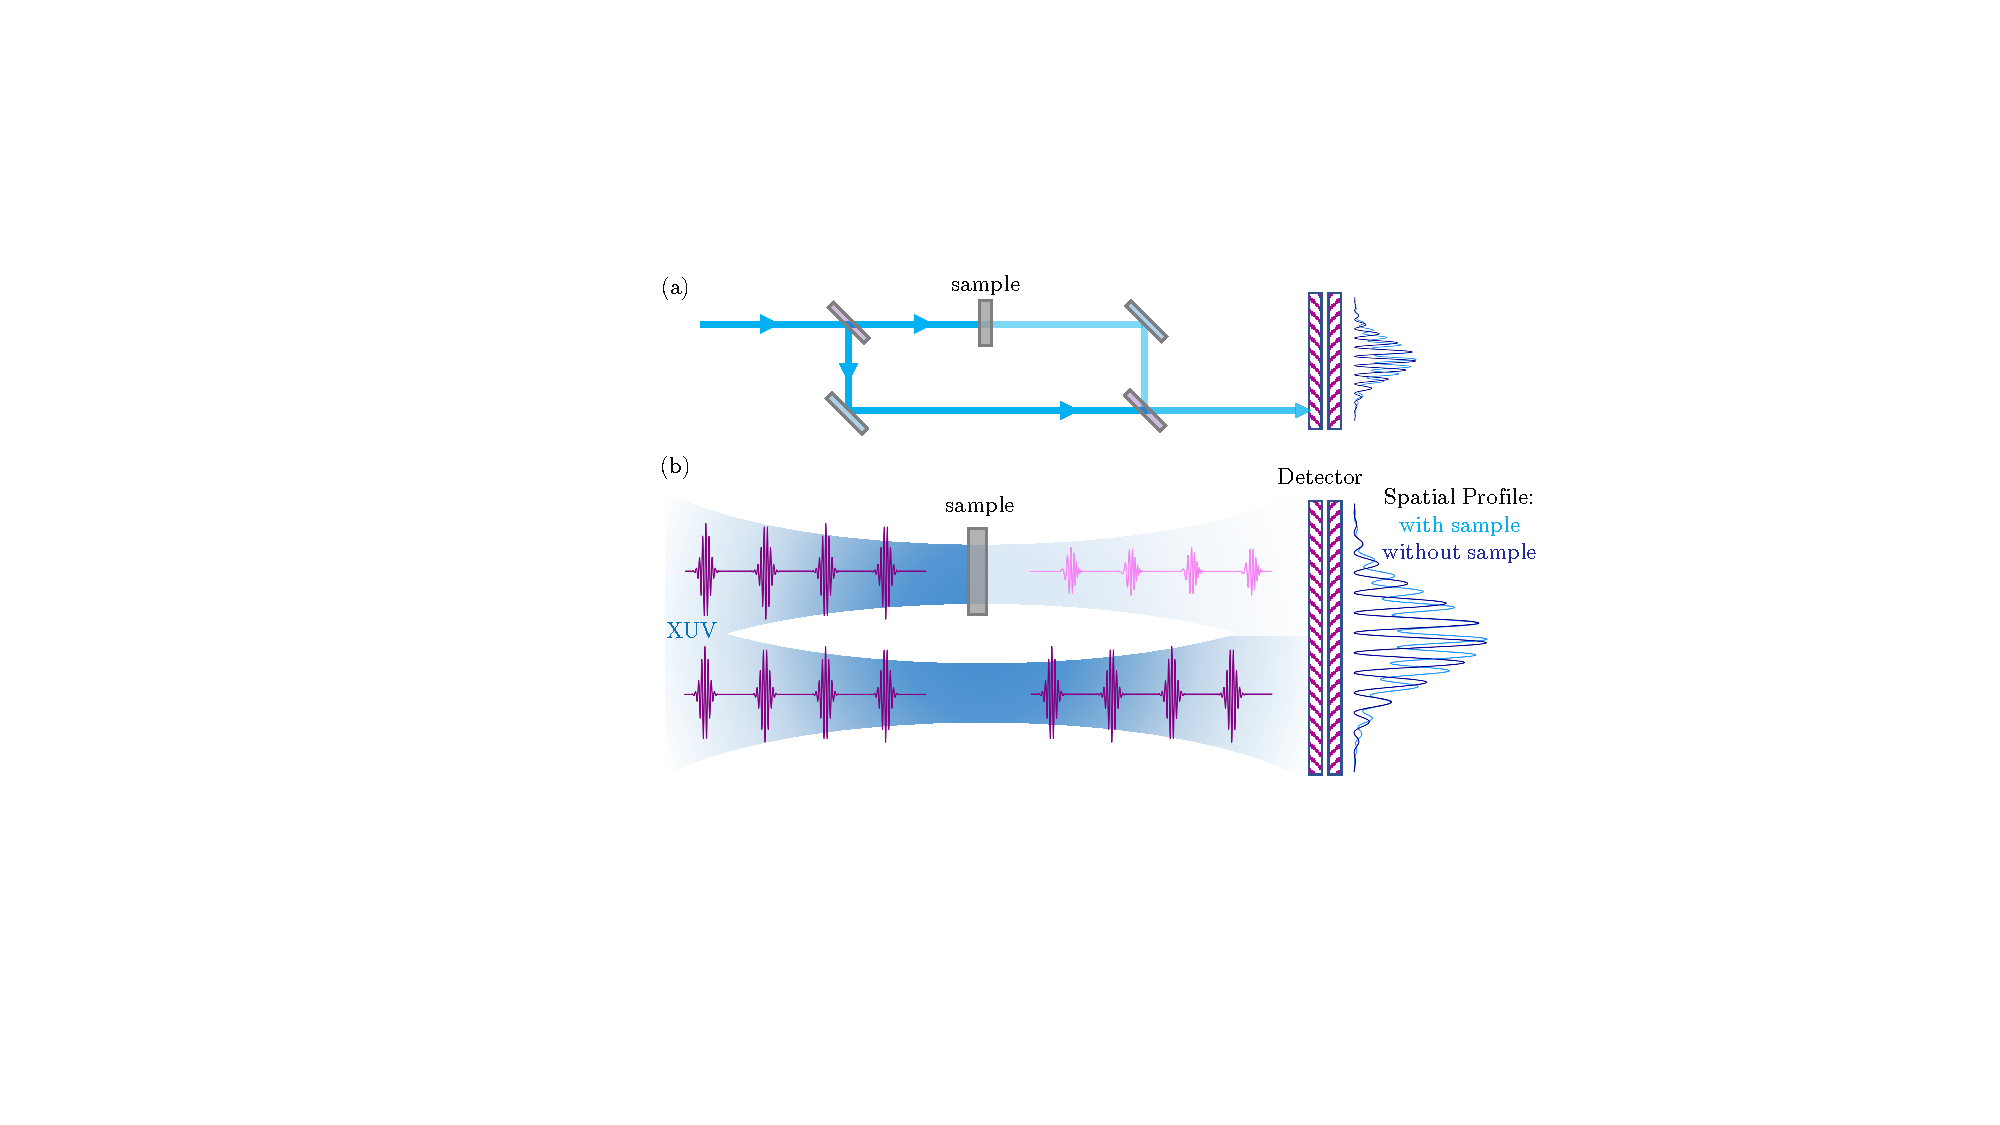
\includegraphics[width=0.8\textwidth]{figures/refractive_index/mach-zehnder_two_source.pdf}
	\caption[Schematic of Mach-Zehnder interferometer and spatial profile with and without a sample in one arm of the interferometer]{(a) Schematic of a Mach-Zehnder interferometer that is used to measure the phase shift induced by a sample placed in one of the arms of the interferometer. (b) For the experiments described in this chapter, the two XUV sources will act as the two arms of a Mach-Zehnder, and the sample of interest will only be introduced into one one the sources.}
	\label{fig:mach-zehnder_interferometer}
\end{figure}

\section{Measurement of the complex refractive index}
\subsection{Experimental setup}
\label{sec:experimental_setup_refrac}
The experimental setup that will be used to demonstrate the ability to measure both the real and imaginary parts of the refractive index is very similar to the experimental setup presented in chapter \ref{chap:two_source}.  The TABLe is the experimental beamline that will be used, and the setup is shown in figure \ref{fig:refract_schematic}.
\begin{figure}
	\centering
	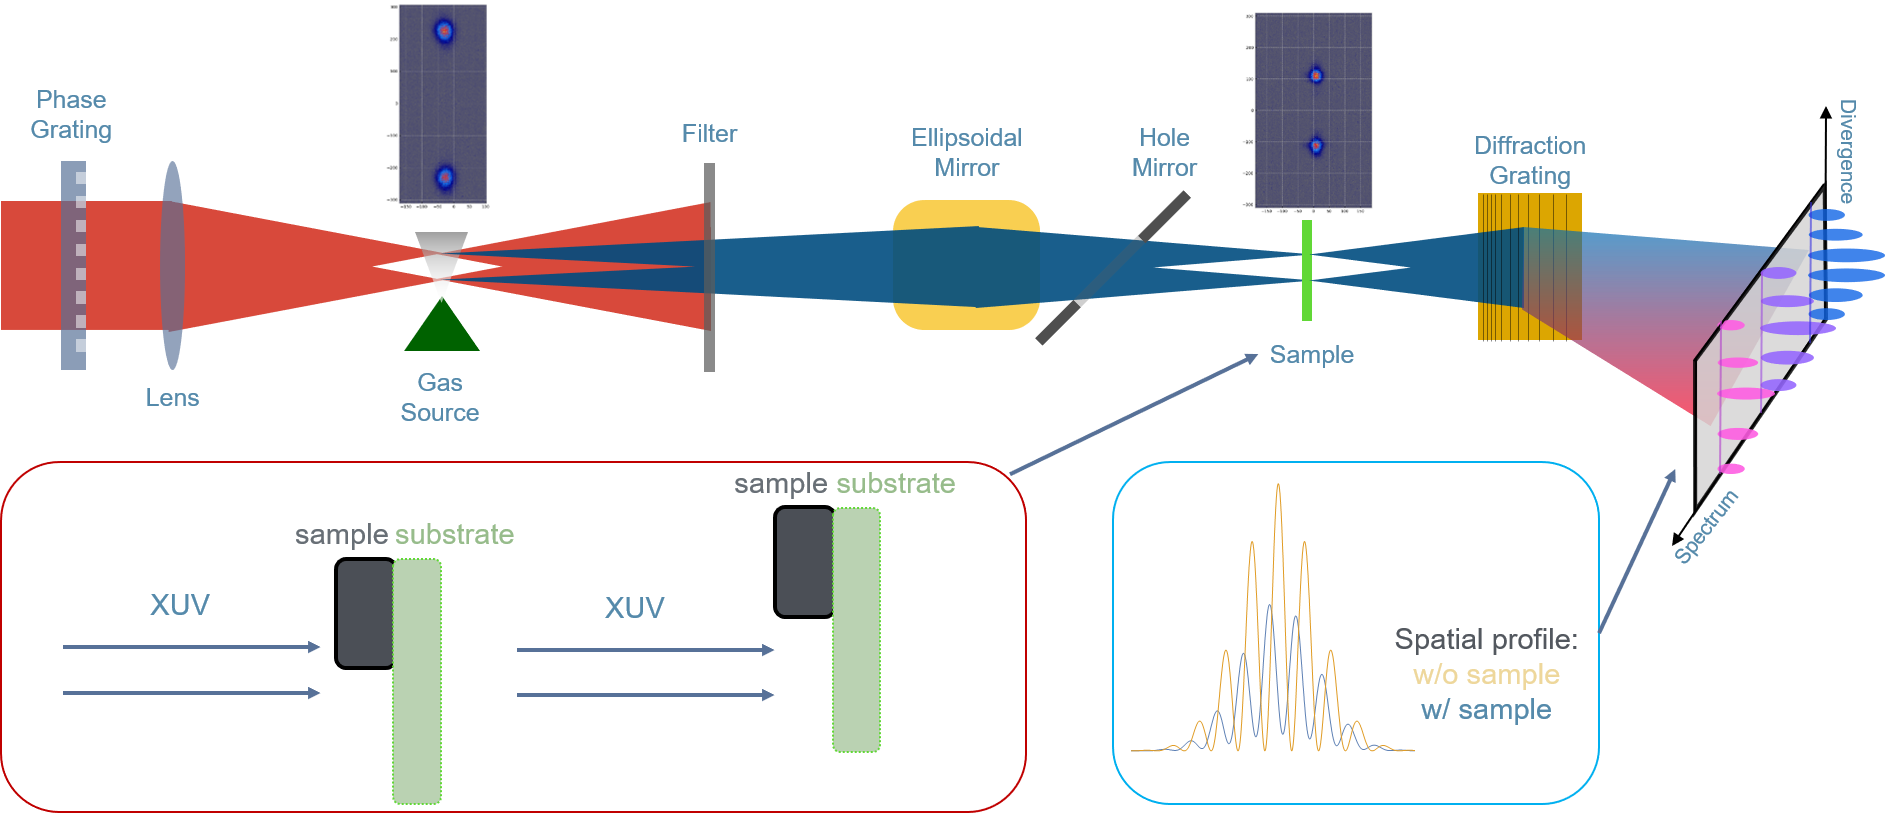
\includegraphics[width=0.8\textwidth]{figures/refractive_index/experimental_setup.png}
	\caption[Schematic of using two-source HHG to measure the real and imaginary part of the refractive index]{Schematic of the two-source HHG experiment performed in the TABLe. A $0-\pi$ SWPG is used to generate two intense lobes at the focus of a lens.  These lobes will generate XUV beams which will interfere in the far-field.  An ellipsoidal mirror is used to refocus the XUV beams into a target chamber before going onto the spectrometer. A sample that is shaped like a step-function will be introduced at the focus of the XUV in the target chamber.  The spatial profile of the various harmonic orders will be measured in the two cases shown.  The fringe shift and fringe contrast changes allow for a simultaneous measurement of both parts of the refractive index of the sample.}
	\label{fig:refract_schematic}
\end{figure}


\begin{figure}
	\centering
	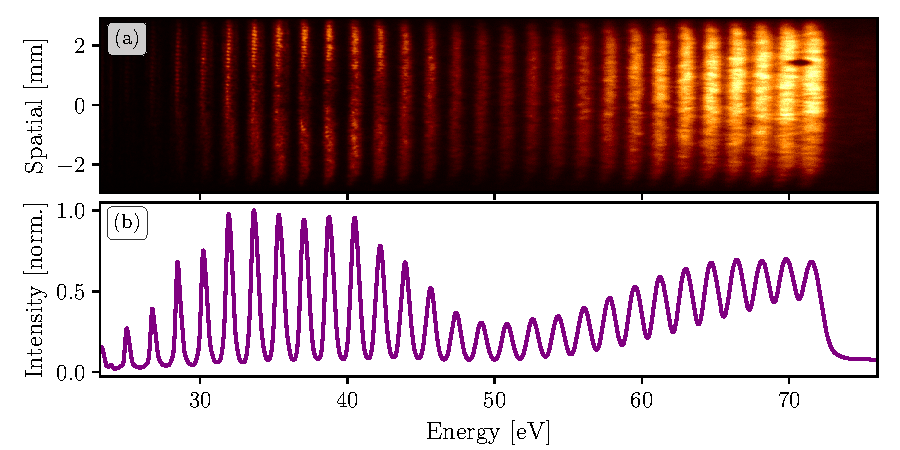
\includegraphics[width=1.0\textwidth]{figures/refractive_index/reference_img_spectrum.pdf}
	\caption[Reference image and spectrum of harmonics used to measure refractive index using SWPG]{Reference image (a) and harmonic spectrum (b) that was used in this experiment.  Fundamental wavelength is 1435 nm, and the harmonics are generated using an SWPG with a period of $d=2.5$ mm.}
	\label{fig:ref_img_spec}
\end{figure}
We use the output of the TOPAS at 1435 nm with a pulse energy of about 2 mJ and a pulse duration of around 60 fs. A $0-\pi$ SWPG is with a grating period of 2.5 mm is used to generate two intense lobes at the focal plane of a 400 mm focal length CaF$_2$ plano-convex lens. At the focal plane, a gas medium is generated by a piezoelectric pulsed gas jet in which harmonics will be generated by the two sources.  The generation gas that will be used is argon. The fundamental wavelength is then filtered out by an aluminum filter.  The Al filter acts a high frequency band-pass with a band-pass region of 20-72 eV for the harmonic energies that are generated at this wavelength. The harmonics are then refocused into a target chamber by an ellipsoidal mirror with a demagnification of three.  This entails that the source separation in the target chamber will be smaller by a factor of three, and the beam waist of each source will also be reduced by a factor of three.  This is where a sample will be introduced into only one of the two XUV sources. The sample in mounted on a motorized stage that allows for control of the position of the sample with respect to the XUV focus. After transmitting through the sample, the XUV will propagate to the spectrometer which allows for the spatial profile of each harmonic order to be measured.  A reference image from the spectrometer and the corresponding harmonic spectrum used in this experiment is shown in figure \ref{fig:ref_img_spec}.

In order to implement the scheme shown in figure \ref{fig:refract_schematic}, we need to introduce a sample into only one of the two XUV sources that are generated.  As mentioned previously, the source separation in the target chamber will be a third of the separation in the generation chamber. For the SWPG and laser parameters that we used for this experiment, the source separation in the harmonic generation chamber is $\Delta x=2\lambda f/d\approx460\:\mu m$, and the corresponding separation will be $\Delta x_t = \Delta x/3\approx153\: \mu m$ in the target chamber.  Therefore, the ideal sample has a cross sectional profile that is as close to a step function as possible, and the width of the step should be much less the separation between the two sources.  In general, this can be accomplished using photolithography techniques to pattern a thin film of the desired profile on top of a free standing membrane substrate.  For one of the samples that is used in this proof of principle experiment, we instead chose to start with a commercially available free standing membrane, and then break the membrane in such a way that it would have a sharp step-like cross sectional profile.  The membrane that was chosen was a free standing 260 nm single crystal Si membrane on a 500 $\mu$m Si frame.  These free standing membranes are manufactured by Norcada.  The sample needs to be this thin because this experiment is done in transmission and XUV is strongly absorbed by most materials. A schematic of the sample that was used is shown in figure \ref{fig:split_sample} (a).  A second sample was also fabricated using e-beam deposition of Ge on top of a 30 nm SiN free-standing membrane.\footnote{This was done by Yaguo Tang, a postdoc in the Agostini-DiMauro group.}  For this sample, shown in figure \ref{fig:split_sample} (b), a physical mask was used to cover half of the SiN membrane before deposition.  Due to the delicate nature of these free-standing membranes, the physical mask could not touch the membrane without breaking it, and this necessitated a small gap between the physical mask and the membrane itself.  The result of this gap is that there will be a more gradual change in thickness between the two halves of the sample (with and without Ge).

\begin{figure}
	\centering
	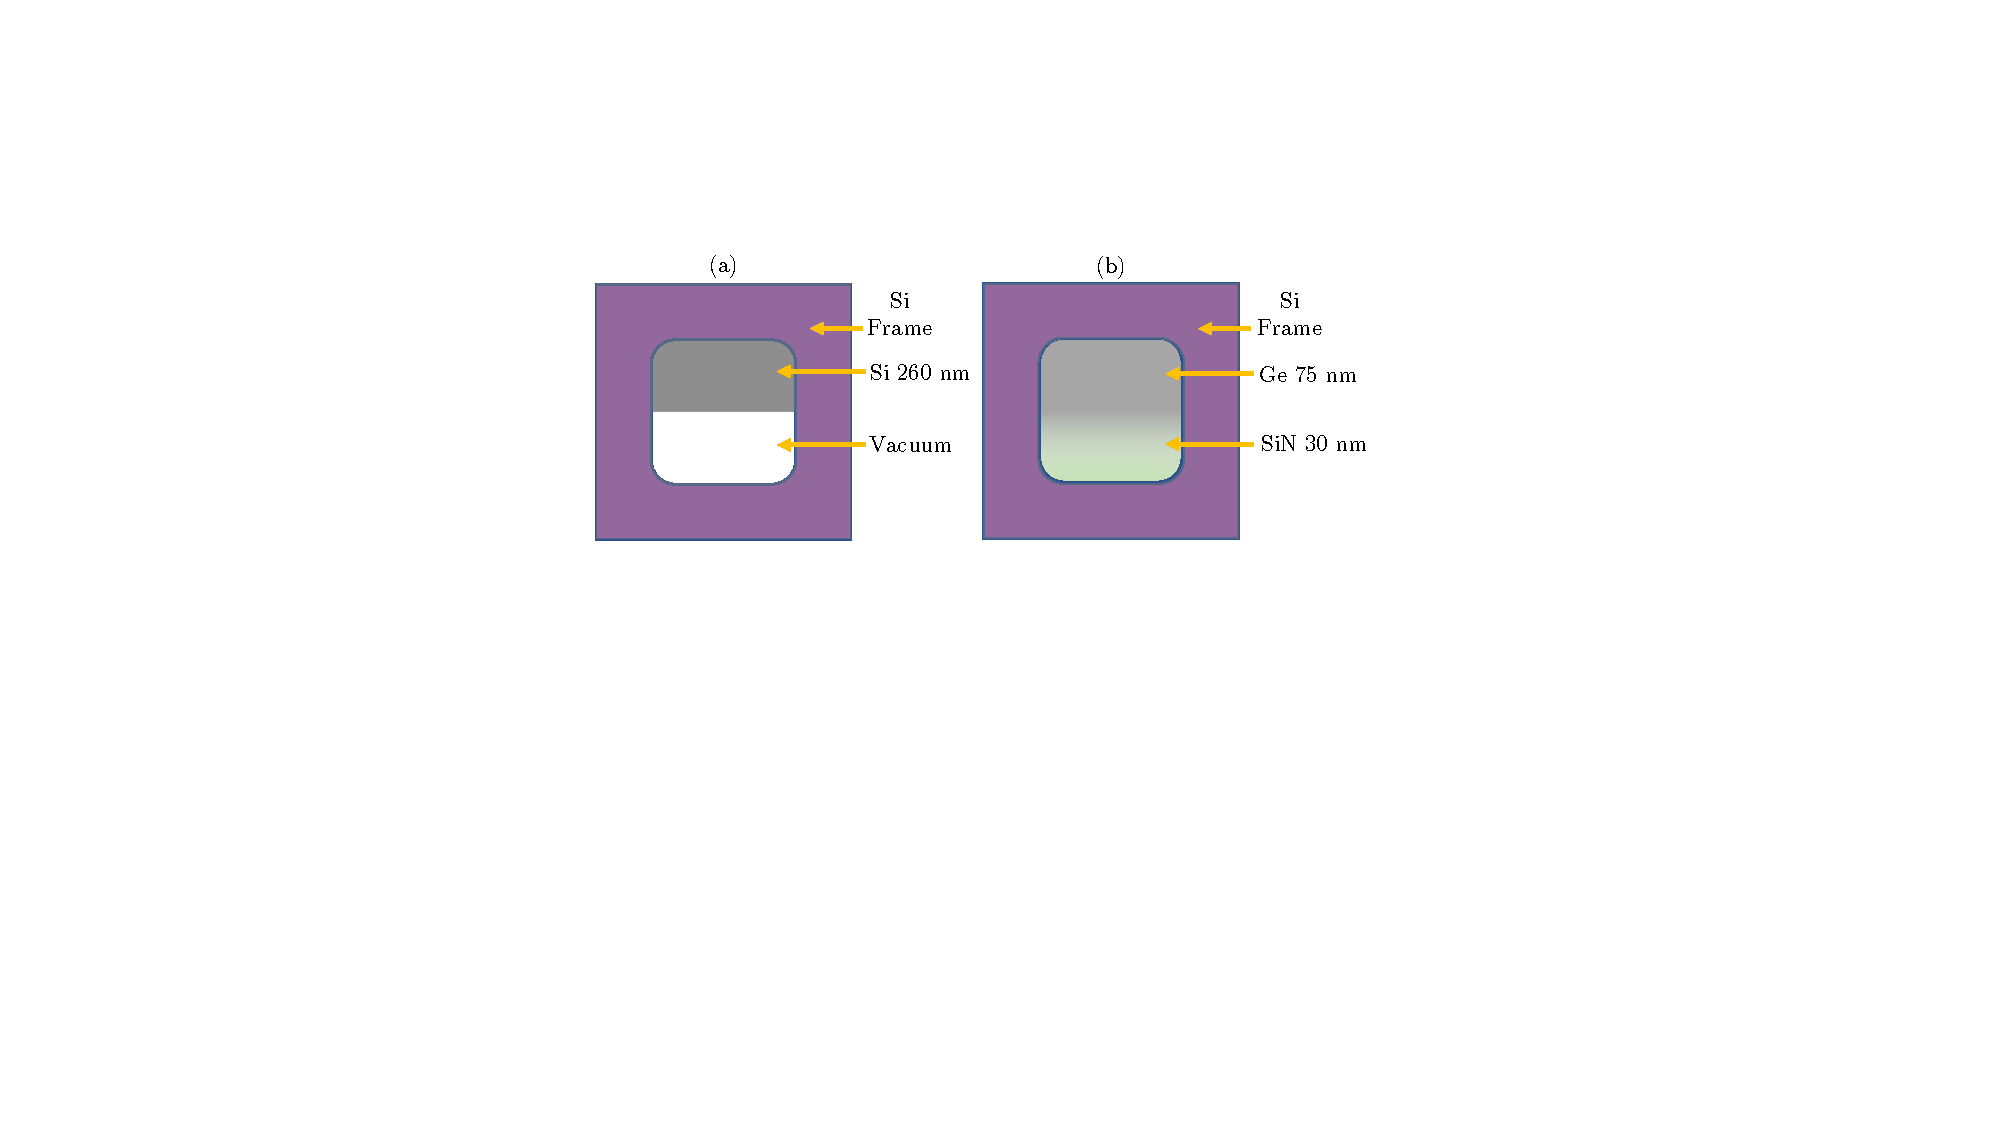
\includegraphics[width=0.8\textwidth]{figures/refractive_index/samples.pdf}
	\caption[Schematic of the samples used to measure the refractive index of silicon and germanium]{Schematic of the samples that were used in this experiment.  (a) Free standing 260 nm Si membrane that has been broken in half.  The way that the sample was cleaved in half ensures that the edge is sharper than the separation between the two sources.  The sample was made by Norcada before it was broken. (b) Germanium deposited on a free standing 30 nm SiN membrane.  E-beam deposition was performed with a physical mask to create a step-like profile.}
	\label{fig:split_sample}
\end{figure}


\begin{figure}
	\centering
	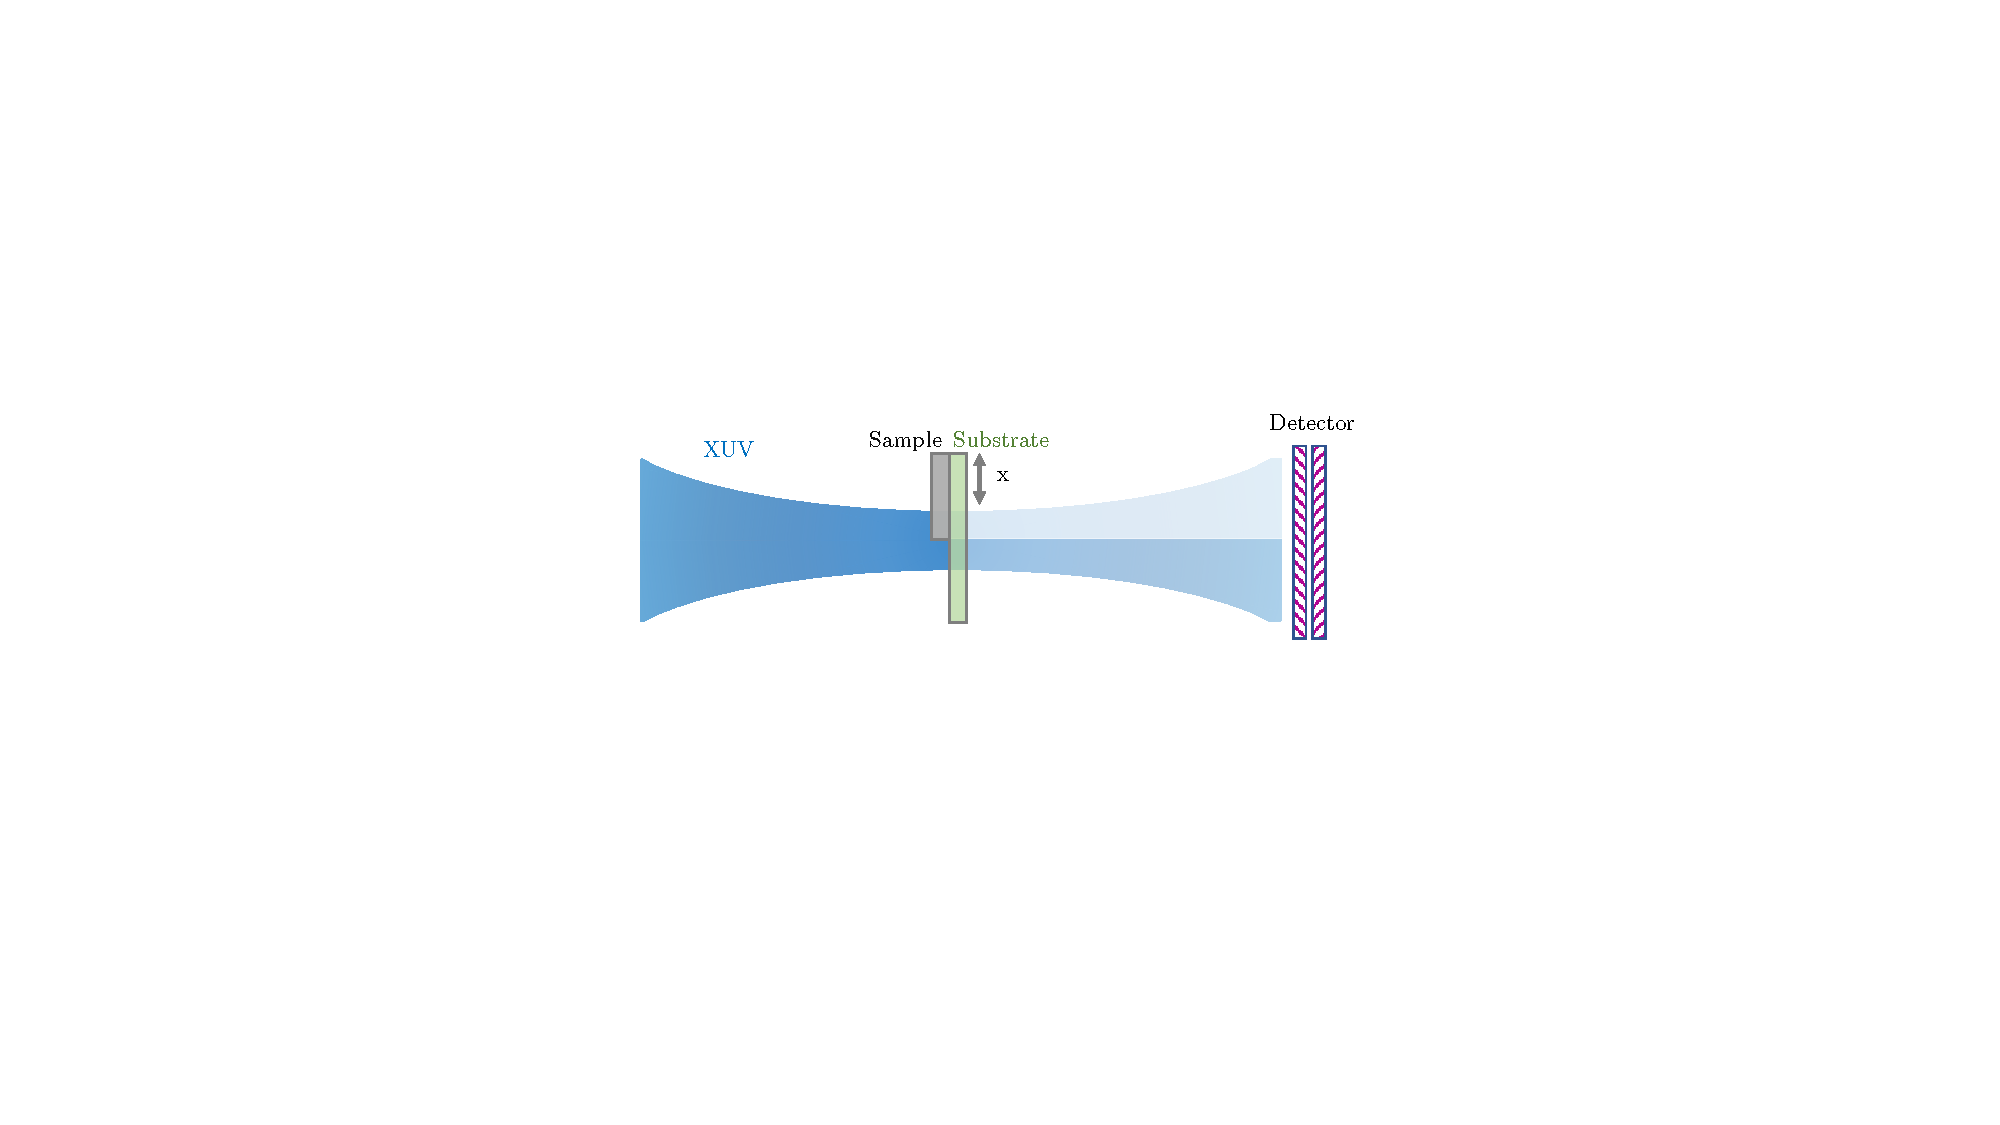
\includegraphics[width=0.7\textwidth]{figures/refractive_index/knife_edge.pdf}
	\caption[Schematic of knife edge technique used as a profilometry tool]{Schematic of knife edge technique used as a profilometry tool.  A transmissive sample and substrate are translated through the focus of the XUV, and the detected harmonic amplitude as a function of position can be used to reconstruct the beam and transmission profiles.}
	\label{fig:knife_edge_schematic}
\end{figure}

To be more precise about the cross sectional profile of the fabricated samples that were used, a form of profilometry was performed using the XUV beam as a probe of the thickness of the sample.  The idea is simply an extension of the knife edge method that is used to measure beam profiles, see section \ref{sec:xuv_beam_size_knife_edge} for the basics.  In this case, the assumption that the knife is totally opaque is lifted and the transmission function of the sample is included.  The total transmitted power in this case now becomes
\begin{equation}
	\label{eqn:transmission_knife_edge_power}
	P(x, \omega) = \int_{\infty}^{\infty}\int_{\infty}^{\infty} T(x - x', \omega) I(x', y')\diff x' \diff y
\end{equation}
where $T(x, E)$ is the transmission of the sample as a function of position and energy.\footnote{For the case of a opaque knife, $T = \Theta(x - x')$ and equation \ref{eqn:knife_edge_power} is recovered.} This essentially represents the spatial convolution of the transmission profile of the sample with the beam profile.  Generally, in order for this to be useful as a profilometry tool, the beam size must be much smaller the feature sizes of the transmission profile.  If this is not the case, then \emph{a priori} knowledge of either the beam profile or the transmission profile is needed to reconstruct the other profile.  As seen in section \ref{sec:xuv_beam_size_knife_edge}, the beam profile can be independently measured using part of the sample frame to determine the beam profile.  If the beam width can be treated as vanishingly small relative to the transmission profile, then the total transmitted power becomes
\begin{equation}
	\label{eqn:knife_edge_delta}
	P(x,\omega) = P_0(\omega)T(x,\omega).
\end{equation}
To determine the thickness profile of the sample some assumptions are need.  If one assumes knowledge of the absorption cross section as a function of energy, then Beer-Lambert's Law can be used directly to calculate the thickness, see equation \ref{eqn:beer-lambert}.  Additionally, if one assumes knowledge of the maximal thickness $d_0$ of the sample on top of the substrate, then the total transmitted power becomes
\begin{equation}
	\label{eqn:trans_power_thickness_assumed}
	P(x,\omega) = P_0(\omega)T(x,\omega) = P_0(\omega)T_0(\omega)^{d(x)/d_0}
\end{equation} 
where $T_0$ is the transmission at the maximal thickness $d_0$.  This allows for calculation of the thickness profile from the integrated harmonic signal, and the resulting relationship is 
\begin{equation}
	\label{eqn:thickness_calc}
	d(x) = d_0\bigg(\frac{\log \overline{C}(x)}{\log \overline{T_0}}\bigg)
\end{equation}
where $\overline{C}$ and $\overline{T_0}$ are the integrated average harmonic counts and maximal transmission.

This method is used to measure the profile of the samples that were used in this experiment.  The results of these measurements are shown in figure \ref{fig:knife_edge_samples}.  The integrated harmonic signal is shown in purple and shows a very sharp step for the Si sample whose width is limited by the harmonic beam waist of 6 $\mu$m, however the Ge sample shows a much broader transition region between the two regions that is approximately 200 $\mu$m in width.  This was to be expected from the type of physical mask used to make the Ge sample, and it could be improved upon by implementing photolithography techniques.  That being said, these samples are of sufficient quality to demonstrate the technique of measuring the complex refractive index using the SWPG.
\begin{figure}
	\centering
	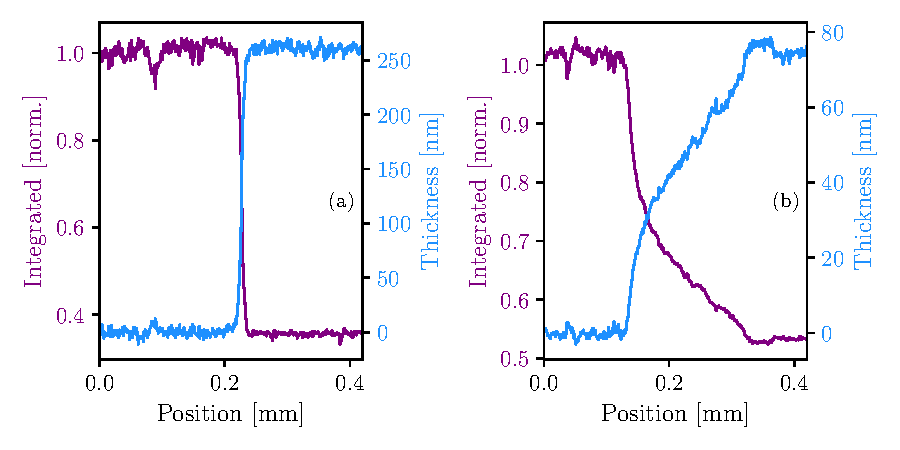
\includegraphics[width=1.0\textwidth]{figures/refractive_index/integrated_knife_edge.pdf}
	\caption[Profilometry using integrated XUV signal for both Si and Ge samples]{Integrated XUV signal (purple) as samples in shown in figure \ref{fig:split_sample} are translated in the focal plane.  Result is a profilometry measurement using XUV to characterize the thickness profile (blue) of the two samples with Si sample shown in (a) and the Ge sample in (b).}
	\label{fig:knife_edge_samples}
\end{figure}

\subsection{Sample Translation}
To measure the complex refractive index of the samples shown in figure \ref{fig:split_sample}, we will look for a fringe shift and change in fringe contrast when only one of the sources is going through the sample and the other is going through either vacuum or the substrate.  To see this, we translate the sample through the focal plane in the target chamber such that three distinct regimes will occur.  The first is when both sources are going through vacuum/substrate, the second is when one source is going the sample and the other is going through vacuum/substrate, and the final regime is when both sources are going through the sample.  Since this is a differential measurement, we would only expect to see a fringe shift for the second regime.  The first and third regimes should show the same fringe pattern, and the only expected difference is the overall modification of the spectral amplitude of the harmonics due the absorption of the sample.  This is shown in figure \ref{fig:harmonic_phase_shift} (b) for the Si sample and figure \ref{fig:harmonic_fringe_shift_contrast_ge} (b) for the Ge sample, where the spatial profile is shown for harmonic order 29 and 37 as the sample is translated through the focal plane.

From the spatial profile shown in figure \ref{fig:harmonic_phase_shift} (b), the three expected regimes can clearly be seen.  There is also additional spatial structure that is present in the transition between each of the three regimes.  This is due to diffraction that is caused by one of the sources being partially blocked.  From the spatial profile, the fringe shift can be extracted from the spatial frequency component that corresponds to this harmonic.  The phase of that spatial frequency is plotted in \ref{fig:harmonic_phase_shift} and shows that there is a phase shift between the two sources when only one of the sources is going the sample.  From this phase shift it is now possible to calculate the real part of the refractive index from the relationship
\begin{equation}
	\label{eqn:fringe_shift_x}
	\delta = \frac{\lambda\Delta\phi}{2\pi\Delta d}
\end{equation}  
where $\Delta d$ is the thickness difference and $\Delta \phi$ is the phase shift between the two sources.  The phase shift that is observed in harmonic order 29 can be seen across the harmonic spectrum, and enables the real part of the refractive index to be extracted across a broad range of photon energies simultaneously.  Similar behaviour is observed for the Ge sample in figure \ref{fig:harmonic_fringe_shift_contrast_ge} (b), however the broad thickness profile of the sample causes a gradual transition between the three regimes as each sources transmits through varying thickness of Ge.  That being said, the phase shift that is observed can still be used to measure the real part of the refractive index, just at an effective thickness given by the difference in thickness of Ge between each source.

\begin{figure}
	\centering
	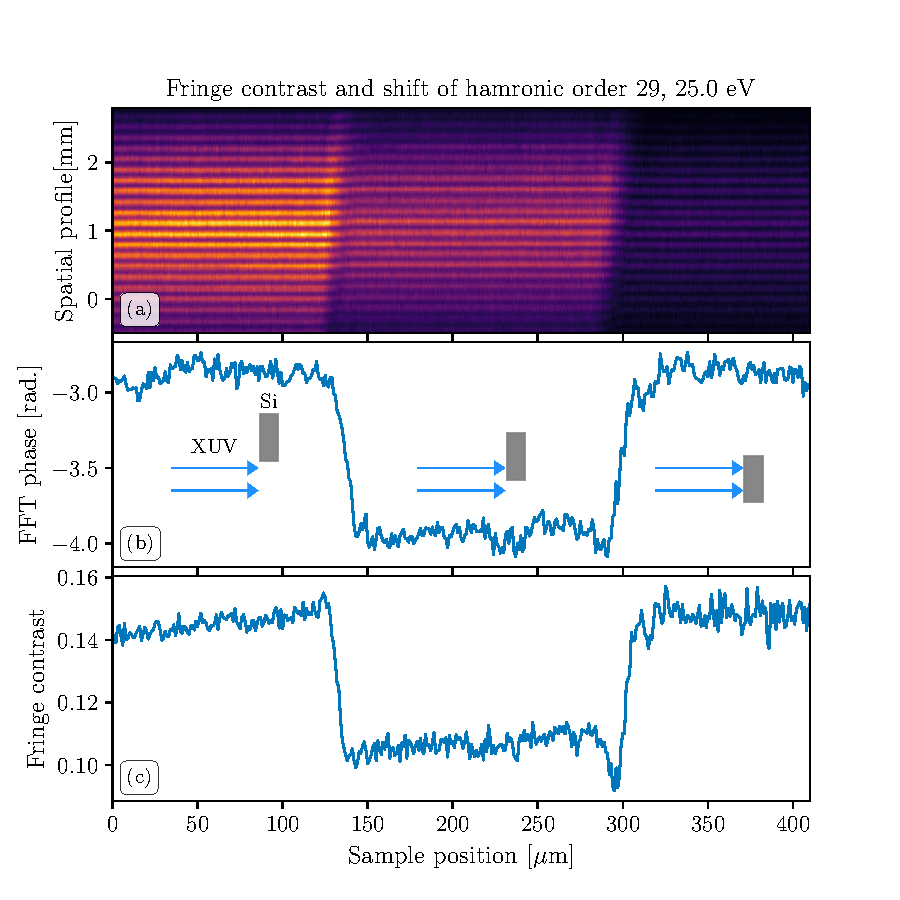
\includegraphics[width=1.0\textwidth]{figures/refractive_index/spatialgram_fringe_shift_contrast.pdf}
	\caption[Spatial profile and fringe shift of a harmonic as sample is translated across the two XUV sources]{(a) Spatial profile of harmonic order 29 as the silicon sample is translated through the two sources. Three regimes are clear from the spatial profile, and they correspond to both sources going through vacuum, only one source going through the sample, and both sources going through the sample.  A clear fringe shift can be seen between the second regime and the other two.  Additional structure is seen at the transition between regimes, and this is due to diffraction cause by the sample partially blocking one of the sources. (b) Phase extracted from the spatial frequency corresponding to this harmonic order.  The phase shift induced by the Si sample can be extracted from this phase shift. (c) Fringe contrast extracted from the spatial frequency corresponding to this harmonic order.}
	\label{fig:harmonic_phase_shift}
\end{figure}

\begin{figure}
	\centering
	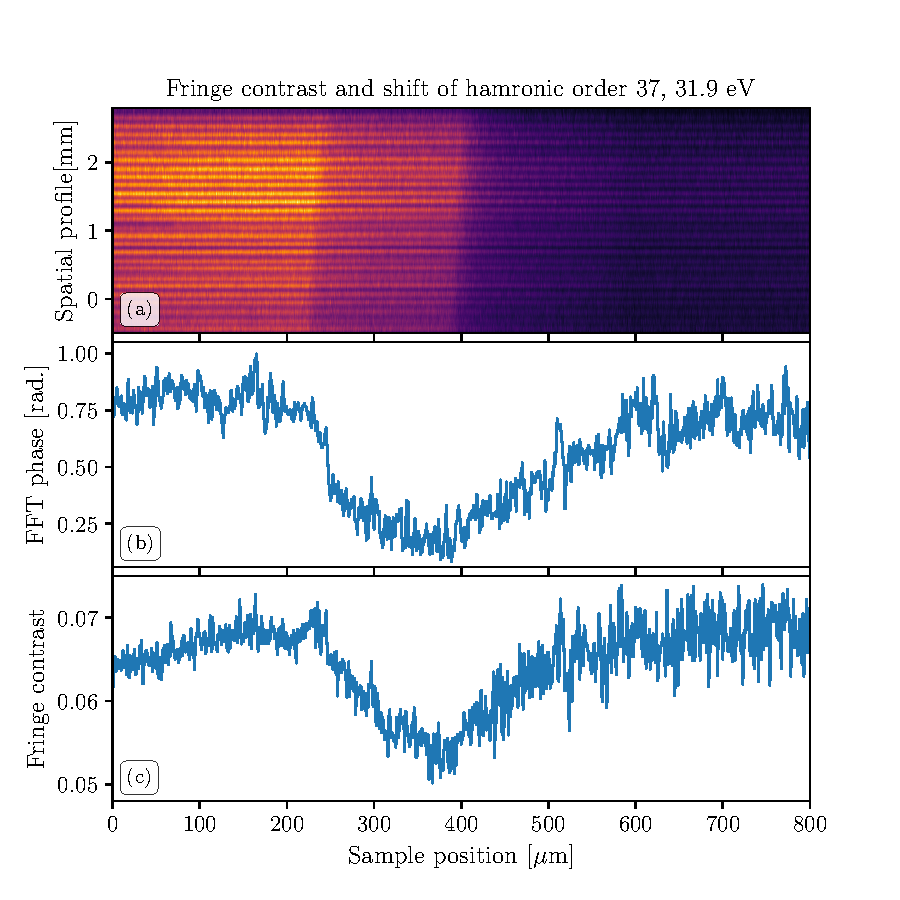
\includegraphics[width=1.0\textwidth]{figures/refractive_index/spatialgram_fringe_shift_contrast_ge.pdf}
	\caption[Spatial profile and fringe shift of a harmonic as sample is translated across the two XUV sources]{(a) Spatial profile of harmonic order 37 as the germanium sample is translated through the two sources. Three regimes are clear from the spatial profile, and they correspond to both sources going through vacuum, only one source going through the sample, and both sources going through the sample.  A clear fringe shift can be seen between the second regime and the other two.  Additional structure is seen at the transition between regimes, and this is due to diffraction cause by the sample partially blocking one of the sources. (b) Phase extracted from the spatial frequency corresponding to this harmonic order.  The phase shift induced by the Si sample can be extracted from this phase shift. (c) Fringe contrast extracted from the spatial frequency corresponding to this harmonic order.}
	\label{fig:harmonic_fringe_shift_contrast_ge}
\end{figure}


In addition to the fringe shift that is show in figure \ref{fig:harmonic_phase_shift} (b), there is also a change in fringe contrast that can be seen as the sample is translated through the two sources.  In general, the fringe contrast can be defined as the relative difference of of the maximum and minimum values of an interference pattern, such that
\begin{equation}
	V=\frac{I_{\mathrm{max}} - I_{\mathrm{min}}}{I_{\mathrm{max}} + I_{\mathrm{min}}} = \frac{I_{\mathrm{amp}}}{I_{\mathrm{mean}}}
\end{equation}
is the fringe visibility or contrast.  When considering the case of two interfering beams, this fringe contrast can be written as
\begin{equation}
\label{eqn:fringe_visibility} 
	V = \frac{2\sqrt{I_1 I_2}}{I_1 + I_2}\rvert\gamma\lvert
\end{equation}
where $I_1$ and $I_2$ are the intensity of the two beams and $\gamma$ is the complex coherence\footnote{The complex coherence is a function of harmonic order $q$ and peak intensity $I_0$ of the fundamental field used to generate the harmonics, and it causes a decrease in fringe visibility for increasing $q$ and $I_0$ \cite{ditmireSpatialCoherenceMeasurement1996}.} \cite{hemmersMulticolorXUVInterferometry2009, ditmireSpatialCoherenceMeasurement1996, wilsonDoubleSlitInterferometry2012}.   
The change in fringe contrast due to the sample translation is shown in figures \ref{fig:harmonic_phase_shift} (c) and \ref{fig:harmonic_fringe_shift_contrast_ge} (c).  The contrast shows the same three distinct regimes that were seen in the fringe shift.  Similarly to the fringe shift, it can be seen that there is only a change in fringe contrast when only one of the sources is going through the sample.  From this contrast, it is possible to calculate the imaginary part of the refractive index.  This can be done using the relationship
\begin{equation}
\label{eqn:beta_fringe_contrast}
	\beta = -\frac{\lambda}{2\pi \Delta d} \ln\Bigg[\frac{V_0}{V}\Bigg(1-\sqrt{1-\bigg(\frac{V}{V_0}\bigg)^2}\Bigg)\Bigg]
\end{equation} 
where $V_0$ is the contrast without the sample and $V$ is the contrast with the sample present in one of the sources \cite{hemmersMulticolorXUVInterferometry2009}.

Therefore, the complex refractive index can be calculated from the apparent fringe shift and change in fringe contrast as the sample is translated through the two XUV sources.  However, this can be improved upon by taking advantage of the unique capability of the SWPG that is used to generate the two sources, and that capability is the ability to control the relative phase between the two sources.  This enables one to measure the complex refractive index using through a Fourier transform spectroscopy technique, and it enables a more accurate measure of the fringe shit and change in fringe contrast induced by the sample.  This method will be discussed in the following section.

\subsection{SWPG Translation}

\begin{figure}
	\centering
	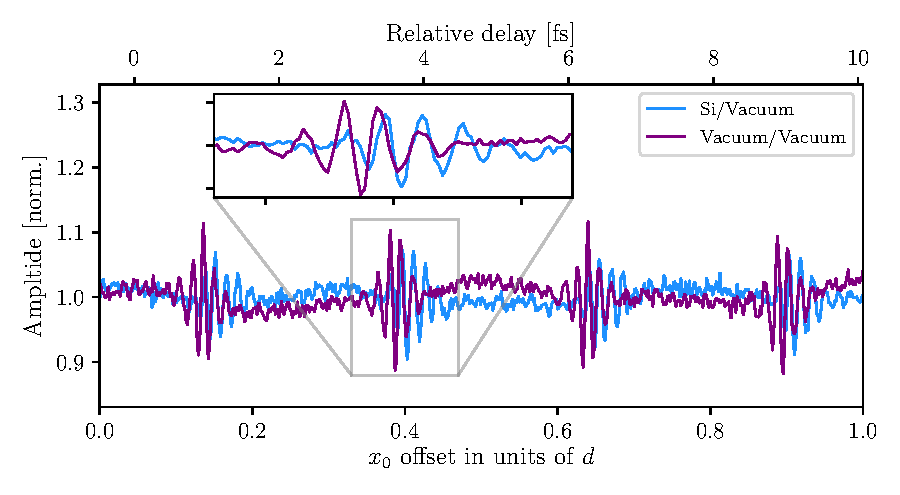
\includegraphics[width=1.0\textwidth]{figures/refractive_index/cross_correlation_si.pdf}
	\caption[Interferogram of all harmonic orders with and without Si sample in one source]{Interferogram of all harmonic orders that is extracted from the combined spatialgram with and without Si sample in one source.  The shift between the two cases is 162 as in relative delay.}
	\label{fig:interferogram_si}
\end{figure}

\begin{figure}
	\centering
	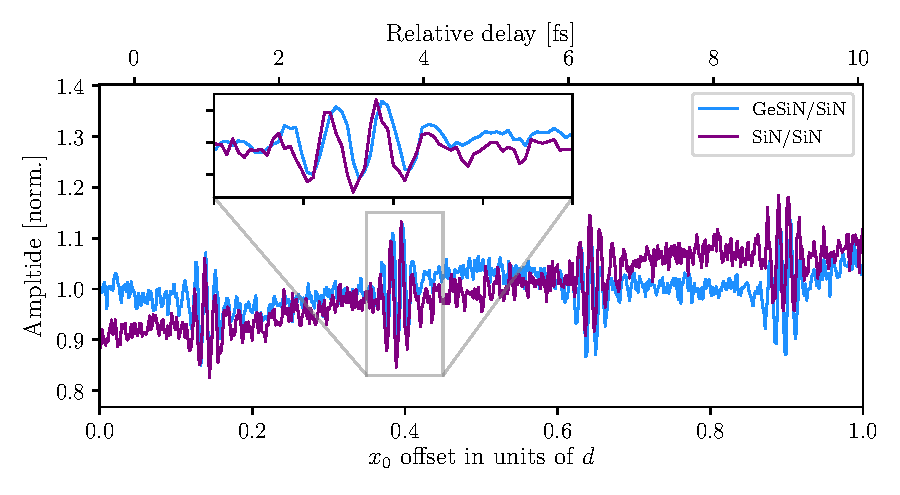
\includegraphics[width=1.0\textwidth]{figures/refractive_index/cross_correlation_ge.pdf}
	\caption[Spatialgram of combined harmonic orders with and without Ge sample in one source]{Spatialgram of combined harmonic orders with and without Ge sample in one source. The shift between the two cases is 16 as in relative delay.}
	\label{fig:interferogram_ge}
\end{figure}



An additional parameter that can be uniquely controlled by using the SWPG is the relative phase between the two XUV sources that are generated, as was established in chapter \ref{chap:two_source}. To leverage this capability, the position of the SWPG can be translated through the beam profile to linearly vary the relative phase between the two sources at two different positions along the thickness profile of the samples.  The obvious candidates for these positions along the thickness profile are: (1) only one source transmits through the sample and the other transmits through the substrate/vacuum and (2) both sources transmitting through the substrate/vacuum.  Intuitively, one would expect to see an additional phase shift between the two sources that is given by equation \ref{eqn:phase_shift}.  To see how this phase shift manifests itself, the interferogram of all harmonic orders that is extracted from the combined spatialgram is shown in figure \ref{fig:interferogram_si} and figure \ref{fig:interferogram_ge} for the two positions in the Si and Ge samples, respectively.  For the case where both sources are going through the vacuum/substrate, this represents the inteferometric autocorrelation of the generated XUV.  For the case where only one source is going through the sample, the combined spatialgram represents a cross-correlation between the reference source and it phase- and amplitude- modulated copy.  Specifically, the detected signal is given by 
\begin{equation}
\label{eqn:combined_spatialgram_theory}
	S(x_0,\omega) = \abs{A_{\mathrm{sample}}}^2 + \abs{A_{\mathrm{ref}}}^2 + A_{\mathrm{sample}}A_{\mathrm{ref}}\exp\bigg(i\bigg(q\frac{4\pi x_0}{d} + \Delta\Phi(\omega)\bigg)\bigg) + c.c.
\end{equation}
where $q=\omega/\omega_0$ is the effective harmonic order, $A_{\mathrm{sample}}$ and $A_{\mathrm{ref}}$ are the amplitudes of the XUV sources going through the sample and reference substrate/vacuum, $\Delta\Phi(\omega)$ is a phase shift between the two sources that includes the phase shift induced by the sample, and $q4\pi x_0/d$ is the phase shift introduced by the SWPG between the two sources \cite{jansenBroadbandExtremeUltraviolet2019}.  In both figure \ref{fig:interferogram_si} and \ref{fig:interferogram_ge}, the structure of the APT can clearly be seen with an attosecond burst every half cycle of the fundamental, and, of more relevance, there is a clear phase shift that can be observed in the spatialgram between the two positions.  To get a sense for the scale of the phase shift seen, the phase imparted by the SWPG between the two sources as a function of grating offset $x_0$ can be interpreted as a relative delay $\Delta t$ between each pulse in the APT when the envelope is broad enough to be neglected.  This yields a relationship given by
\begin{equation}
	\label{eqn:phase_to_delay}
	\Delta t  = \bigg(\frac{\lambda_0}{c}\bigg)\bigg(\frac{x_0}{d}\bigg)
\end{equation}
where $\lambda_0$ is the fundamental wavelength used to generate the two XUV sources. This delay corresponding to $x_0$ is also shown in figures \ref{fig:interferogram_si} and \ref{fig:interferogram_ge}, and the apparent shift between the two cases is 162 as for the Si sample and 16 as for the Ge sample.  The ability to measure such a small shift highlights the capabilities of the SWPG because its inherent stability as a single optic interferometer enables this type of measurement.  Additionally, a step size of 1 $\mu$m in $x_0$ that is easily achieved with many motors yields a relative delay of 1.9 as for $\lambda_0=1435$ nm and $d=2.5$ mm, so this level of precision is easily obtained. 

\begin{figure}
	\centering
	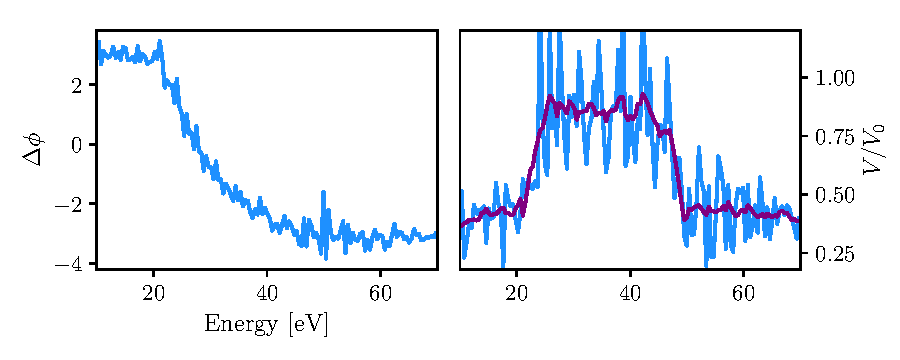
\includegraphics[width=1.0\textwidth]{figures/refractive_index/FTS_delta.pdf}
	\caption[Measured phase shift using SWPG FTS in silicon]{Spectral phase shift extracted from interferograms shown in figure \ref{fig:interferogram_si}. Phase shift is induced by the Si sample.  Smoothed signal is shown using a Savitzky–Golay filter, and this is used in further calculations to extract the refractive index.}
	\label{fig:FTS_phase_si}
\end{figure}

\begin{figure}
	\centering
	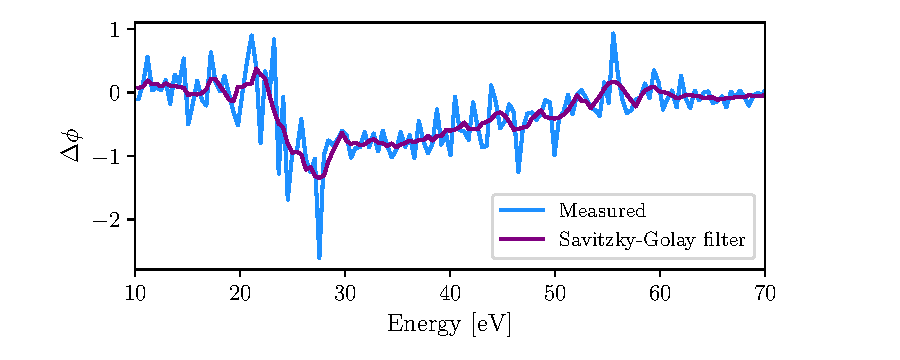
\includegraphics[width=1.0\textwidth]{figures/refractive_index/FTS_delta_ge.pdf}
	\caption[Measured phase shift using SWPG FTS in germanium]{Spectral phase shift extracted from interferograms shown in figure \ref{fig:interferogram_ge}. Phase shift is induced by the Ge sample. Smoothed signal is shown using a Savitzky–Golay filter, and this is used in further calculations to extract the refractive index.}
	\label{fig:FTS_phase_ge}
\end{figure}

From the interferograms shown in figures \ref{fig:interferogram_si} and \ref{fig:interferogram_ge}, it is possible extract the spectrally dependent phase shift that is imparted by the sample.  This is possible because those inteferograms constitute a Fourier-transform spectroscopy (FTS) measurement in the XUV using two phase locked beams generated by a SWPG.  FTS enables measurement of both the real and imaginary parts of the refractive index, however it is difficult to perform in the XUV because of technical requirements set by the available optics and because the intrinsically short wavelengths in this energy range require high interferometric stability and precise control over the relative delay between the interfering beams \cite{jansenSpatiallyResolvedFourier2016, jansenBroadbandExtremeUltraviolet2019, kovacevExtremeUltravioletFourierTransform2005, deoliveiraHighresolutionBroadbandwidthFouriertransform2011}.  Both of those difficulties are solved through the use of a SWPG to generate the two sources that are used in this measurement.  To extract the induced phase, the signal given by \ref{eqn:combined_spatialgram_theory} is Fourier transformed using the relative delay given by \ref{eqn:phase_to_delay}, and this yields
\begin{equation}
	\label{eqn:spatialgram_theory_FT}
	\tilde{S}(\omega) = A_{\mathrm{sample}}A_{\mathrm{ref}}\exp\big(i\Delta\Phi(\omega)\big).
\end{equation}
In principle, the phase $\Delta\Phi$ includes geometric phase variations and phase variations from the HHG process \cite{jansenBroadbandExtremeUltraviolet2019}.  To remove these contributions, a reference interferogram should be taken to isolate the phase contribution from the sample of interest, and this is precisely what was done by scanning the SWPG in the two positions mentioned previously.  The sample induced phase $\Delta\phi$ is calculated from \ref{eqn:spatialgram_theory_FT} for both positions through the relationship
\begin{equation}
	\label{eqn:measured_spectral_phase}
	\Delta\phi(\omega) = \arg\big[ \tilde{S}_{1}(\omega) \tilde{S}_{2}^{\ast}(\omega) \big]
\end{equation}
where $\tilde{S}_{1}(\omega)$ is the Fourier transformed interferogram measured at a position where only one source is on the sample and $\tilde{S}_{2}^{\ast}(\omega)$ the complex conjugate of the Fourier transformed interferogram measured at a position where neither source is on the sample of interest \cite{jansenBroadbandExtremeUltraviolet2019}.  This analysis was performed to extract the phase shift induced by the Si and Ge samples shown in figure \ref{fig:split_sample}, and the resulting phase shift is shown in figure \ref{fig:FTS_phase_si} (a) for the Si sample and figure \ref{fig:FTS_phase_ge} (a) for the Ge sample. Additionally, a smoothed signal is shown using a Savitzky-Golay filter in both figures. The phase induced by the Si sample shows a decreasing phase shift as the energy is increased with no apparent resonant structure, and this is expected for Si because there are no absorption edges corresponding to a core-level transition in this energy range \cite{henkeXRayInteractionsPhotoabsorption1993}.  The phase shift induced by the Ge sample, on the other hand, shows a pronounced resonance feature around 30 eV.  This feature can be assigned to the $M_{4,5}$ absorption edge due to a core-level transition from the $3d$ states to states in the vicinity of the Fermi energy \cite{henkeXRayInteractionsPhotoabsorption1993, kaplanRetrievalComplexvaluedRefractive2019, borjaExtremeUltravioletTransient2016, krausAttosecondTransientReflectivity2016, zurchDirectSimultaneousObservation2017, zurchUltrafastCarrierThermalization2017}. The signal is noisier in this case when compared to the Si sample because of the overall lower sample quality and the comparatively weaker harmonics in this energy range because of the absorption resonance and absorption from the substrate which does not contribute to the measured phase.  This could be improved by fabricating a thinner sample with a more step-like thickness profile on a thinner membrane or by fabricating a free-standing membrane of Ge similar to the Si sample.


Beyond the sample induced phase shift, FTS can also give access to the imaginary part of the refractive index and thereby the energy dependent transmission of the sample.  This can be calculated from the interferograms at the two positions along the sample using the relationship
\begin{equation}
	\label{eqn:transmission_s1_s2}
	\begin{aligned}
		T(\omega) &= \frac{A_{\mathrm{sample}}(\omega)}{A_{\mathrm{ref}}(\omega)} = \frac{A_{\mathrm{sample}}(\omega)A_{\mathrm{ref}}(\omega)}{A_{\mathrm{ref}}(\omega)A_{\mathrm{ref}}(\omega)}\\
						&=\frac{\abs{\tilde{S}_1(\omega)}}{\abs{\tilde{S}_2(\omega)}}.
	\end{aligned}
\end{equation}
Applying this calculation to the interferograms measured for both samples is shown in figure \ref{fig:FTS_phase_si} (b) and \ref{fig:FTS_phase_ge} (b) for Si and Ge, respectively.  As can be seen from these figures, the transmission is noisier than the induced phase, however several features can still be observed in the energy range of 20-45 eV.  In the case of Si, there is an increasing transmission that plateaus as the energy is increased.  The drop is transmission past 45 eV is likely an artifact of the poor fringe contrast in the harmonics generated above 45 eV.  This general behaviour agrees well with what is expected for Si \cite{henkeXRayInteractionsPhotoabsorption1993}.  For the case of Ge, the signal is even noisier than that of Si, however there is still a drop on transmission at 30 eV that corresponds to the $M_{4,5}$ absorption edge.

\begin{figure}
	\centering
	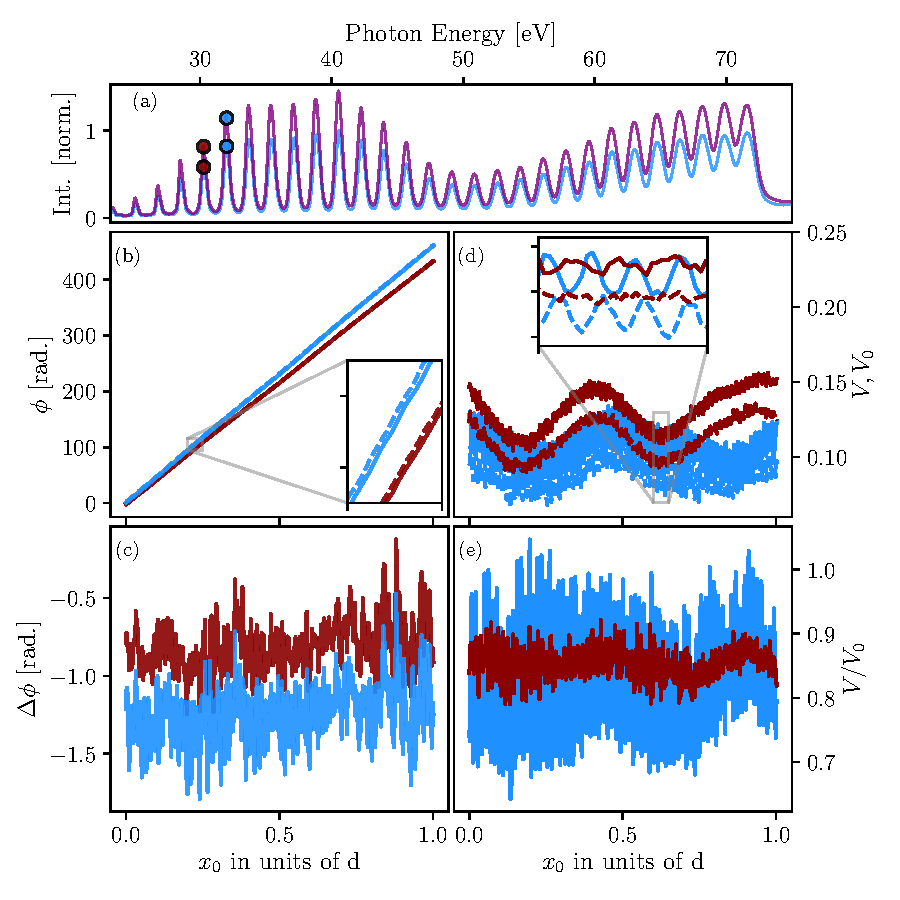
\includegraphics[width=1.0\textwidth]{figures/refractive_index/phase_fringe_extraction.pdf}
	\caption[Fringe shift and fringe  contrast extracted from SWPG scan]{(a) Reference harmonic spectrum showing the two harmonics of interest. (b) Phase of the spatial frequency corresponding to the two harmonics of interest. (c) Difference in phase between the positions along the sample thickness profile. (d) Fringe contrast of each harmonic for the two positions along the sample.  (e) Ratio of fringe contrast between the two positions.}
	\label{fig:phase_fringe_extraction}
\end{figure}

An additional way to extract the spectral phase and transmission induced by the sample is by examining the fringe shift and contrast as the grating position is varied in a similar manner as to what was done while the two samples were translated through the focus of the XUV, see figures \ref{fig:harmonic_phase_shift} and \ref{fig:harmonic_fringe_shift_contrast_ge}.  This can be done for each harmonic as $x_0$ is varied at the two positions along the sample thickness profile.  The resulting fringe shift and contrast can then be averaged to give a measurement of the induced phase shift and absorption of the sample across the harmonic spectrum.  This is shown for two harmonics in figure \ref{fig:phase_fringe_extraction} for the Si sample.  The phase $\phi$ corresponds to the phase of the spatial frequency of the harmonic, and it varies linearly with grating position $x_0$ via the relationship
\begin{equation}
	\phi=\bigg(q\frac{4\pi}{d}\bigg)x_0 + \phi_0.
\end{equation} 
As can be seen in the figure, the phase offset is different for the two positions where only one source is transmitting through the sample (solid line) and where neither sources are transmitting through (dashed line).  The difference in phase between these two cases is precisely the sample induced phase that measured previously by the FTS method, and the phase difference $\Delta\phi$ can be averaged over $x_0$ to give a more accurate phase shift at that harmonic energy. 

In a similar way to the fringe shift, the fringe contrast can be measured as the phase grating is translated for the two sample positions. The resulting fringe contrast is shown in figure \ref{fig:phase_fringe_extraction} (d) for the position where only one source transmits ($V$, dashed line) and where neither source does ($V_0$, solid line).  As expected, the fringe contrast is greater for the case where neither source transmits through the sample because of the differential nature of this measurement.  The modulations that are observed in the contrast as the SWPG is translated through the beam are due to interferences between the two sources in generation of the XUV beams.  The leakage of one IR source into the other causes the slower modulations with a period of $d/2$, and the higher frequency modulations are due to interferences between the two sources at the harmonic energy.  Regardless of their origin, the relevant quantity to extract the absorption induced by the sample is related to the ratio of contrasts $V/V_0$, see equation \ref{eqn:beta_fringe_contrast}, and averaging $V/V_0$ over $x_0$ gives a more accurate change in fringe contrast. 


Finally, we can now calculate both the real and imaginary part of the refractive index of Si and Ge over the range 25 - 60 eV by combining both the fringe shift and the change in fringe contrast and by using the FTS method.\footnote{For the FTS method, the signal smoothed by a Savitzky-Golay filter is used. See figures \ref{fig:FTS_phase_si} and \ref{fig:FTS_phase_ge}.}  The results are shown in figure \ref{fig:measured_delta_beta} for Si and figure \ref{fig:measured_delta_beta_ge} for Ge.  As can be seen in the figure \ref{fig:measured_delta_beta}, there is excellent agreement between the measured real and imaginary parts of the refractive index of Si when compared to the values that can be obtained from CXRO \cite{henkeXRayInteractionsPhotoabsorption1993}.  Both methods agree exceedingly well across most of the energy range of interest for the real part of the refractive index, however there are deviations between the FTS method (blue line) and the average fringe shift (purple dots) at energies above 45 eV.  This is most likely due to the poor fringe contrast at energies above 45 eV, as seen in figure \ref{fig:ref_img_spec} (a).  This deviation between the two methods is most pronounced in the imaginary part $\beta$ shown in figure \ref{fig:measured_delta_beta} (b).  In principle, this measurement can be improved by generating harmonics with good contrast over the entire energy range of interest, and this can most easily be accomplished by using a grating with a larger period to reduce the overall spatial frequencies.

\begin{figure}
	\centering
	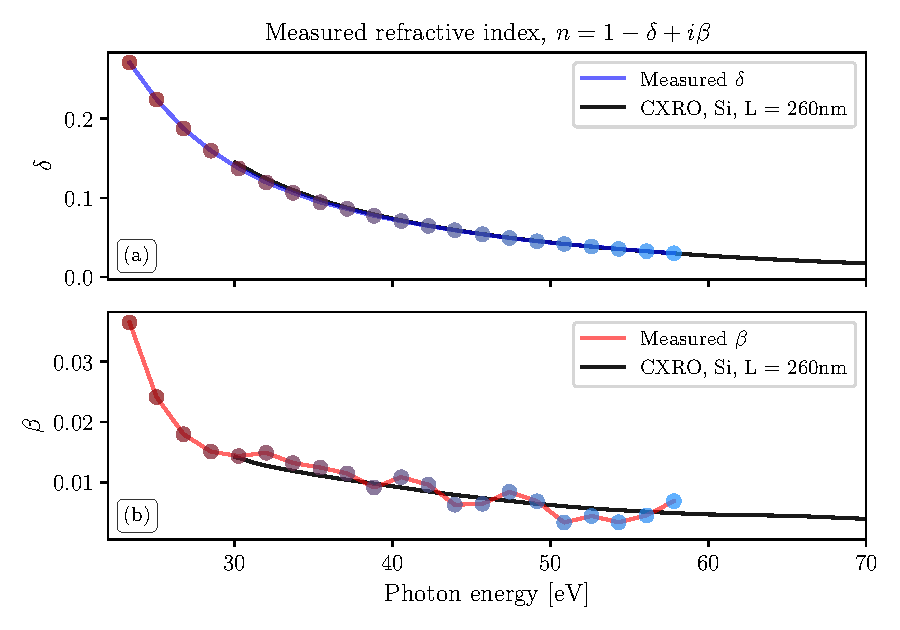
\includegraphics[width=0.9\textwidth]{figures/refractive_index/db_cxro.pdf}
	\caption[Measured real and imaginary part of the refractive index of Si using a SWPG]{Real (a) and imaginary (b) part of the refractive index of Si measured with a SWPG using FTS (blue line) and averaging fringe contrast (FC) and fringe shift (FS) over $x_0$ (purple dots).}
	\label{fig:measured_delta_beta}
\end{figure}

\begin{figure}
	\centering
	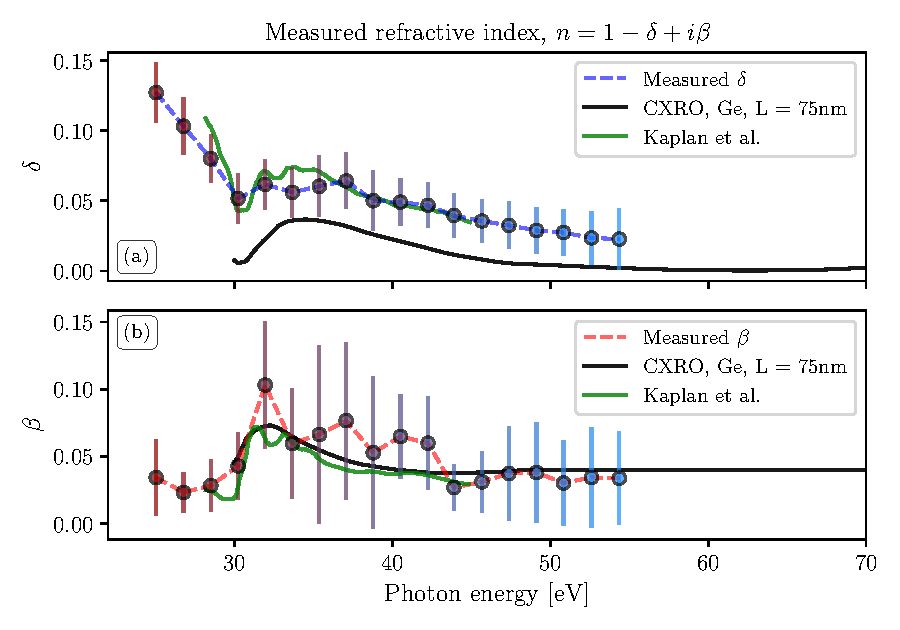
\includegraphics[width=0.9\textwidth]{figures/refractive_index/ge_refractive.pdf}
	\caption[Measured real and imaginary part of the refractive index of Ge using a SWPG]{Real (a) and imaginary (b) part of the refractive index of Ge measured with a SWPG using FTS (blue line) and averaging fringe contrast (FC) and fringe shift (FS) over $x_0$ (purple dots).}
	\label{fig:measured_delta_beta_ge}
\end{figure}

In this energy range, the Si refractive index is devoid of any resonance features because there no nearby absorption edges, so its measurement represents an easy benchmark of both methods of extracting the refractive index. However, what is typically of interest in most experiments is the refractive index at an absorption edge where there is strong variation in refractive index that is intrinsically related to the properties of the material in question.  This is where the measurement of the refractive index of Ge, as shown in figure \ref{fig:measured_delta_beta_ge}, comes in to play.  As mentioned previously, the $M_{4,5}$ absorption edge in Ge is located at 30 eV, and its presence causes a large increase in absorption and a modulation of the phase around the absorption edge.  The refractive index that has been tabulated by CXRO generally is only accurate far from such resonance features. However, recent measurements of the refractive index were performed by Kaplan, \emph{et. al.} \cite{kaplanRetrievalComplexvaluedRefractive2019}, and this measurement serves as a good comparison to the two measurements methods presented herein.  As can be seen from figure \ref{fig:measured_delta_beta_ge}, there is generally excellent agreement between the two measurement methods and  Kaplan, \emph{et. al.} for the real part of the refractive index over the entire energy range of interest, however there are small deviations just above the edge between them. In this energy range just above the edge, the material properties of the sample strongly influence the refractive index, and further study of the sample properties could explain the deviations \cite{kaplanRetrievalComplexvaluedRefractive2019, stohrNEXAFSSpectroscopy1992, attwoodSoftXraysExtreme2000}.  Similarly to the real part of the refractive index, the imaginary part, see figure \ref{fig:measured_delta_beta_ge} (b), shows good overall agreement from 30 - 45 eV in the vicinity of the absorption edge with small deviations that could possibly be explained with further analysis.  However, for the imaginary part, the FTS fails outside the energy range of 30-45 eV because of a noisy signal.  This could be improved both by fabricating a higher quality sample with a more suitable thickness profile and by optimizing the harmonics for better contrast over a larger energy.  Regardless, this demonstrates the feasibility of using a SWPG to measure the complex refractive index over a large energy range in a single measurement even when a resonant feature is present.



\section{Conclusion}
In this chapter, the complex refractive index was introduced and a method to measure both the real and imaginary parts was proposed. The method relies on the use of a $0-\pi$ SWPG to generate two relative phase locked XUV sources whose interference acts as an inline Mach-Zehnder interferometer.  By introducing a sample into one of the sources, the corresponding fringe shift and change in fringe contrast gives access to the real and imaginary parts of the refractive index. The intrinsic phase control offered by the SWPG allows for FTS to be performed by varying the SWPG position within the beam. Samples of Si and Ge were fabricated to test this method, and measuring their refractive index shows excellent agreement between our measured results and the literature. Thus, we have demonstrated the capability of using a SWPG to characterize the ground state complex refractive index of a condensed matter system.  The next step is to extract the dynamic real and imaginary parts that are induced by dressing the sample with another IR field.  This will be discussed in a later chapter.



